\message{ !name(xml.tex)}
\message{ !name(xml.tex) !offset(-2) }

\subsection{Les bases du formalisme XML}

\begin{frame}[allowframebreaks,containsverbatim]{Un document XML}

\begin{center}
\begin{minipage}{0.7\textwidth}
\lstinputlisting[basicstyle=\tiny, language=XML,breaklines=true, caption={Un simple fichier XML}]{codes/exemple_simple.xml}
\end{minipage}
\end{center}

\prof{Document texte lisible.\\
Prologue : version XML, encodage du texte (jeu de caract\`eres). Entre $<?$ et $?>$\\
Optionnel : par d\'efaut, 1.0 et UTF-8\\
Manque les instructions de traitement (informations destin\'ees à l'application cible), qui permettent par exemple d'associer une feuille de style XSL (on verra ça plus tard). Entre <? ?> aussi lais diff\'erent du prologue.\\
}

\framebreak

Un document XML est compos\'e de :


\begin{enumerate}
\item Un prologue 
\begin{enumerate}
\item d\'eclaration de document XML \verb7<?xml version = "1.x" [encoding = "norme" ][standalone = "yes/no" ]? >7  \prof{encoding par d\'efaut : UTF-8.
Version : 1.1 : diff\`ere avec des fonctionalit\'e suppl\'ementaires concernant des caract\`eres "sp\'eciaux" (genre fin de ligne "ascii"). Conseill\'e que si besoin de ces fonctionnalit\'es suppl\'ementaires; en gros, quasi tout le monde travaille en 1.0
2.0 à l'\'etude\\
Standalone, relevant que si une DTD est d\'eclar\'ee en interne du document. Attribut g\'en\'eralement omis car optinnel.
Default = no. it is a signal to the XML processor that the DTD is not just for validation: there could be things to look up in the DTD like:Default values for attributesEntity declarations.
}
\item suivie \'eventuellement (sans contrainte d’ordre) 
\begin{itemize}
\item d’une d\'eclaration ou (exclusif) une r\'ef\'erence à une DTD \verb7<!DOCTYPE element racine [schema racine ] >7 ou \verb7<!DOCTYPE element racine SYSTEM "uri schema racine" >7 
\item de commentaires \verb?<!-- texte --> ?
\item d’instructions de traitement (par ex. appel à XSLT) \verb7<?instruction attribut1 = "valeur" ... attribut n ="valeur" ? >7 \prof{Instruction de traitement, par exemple en HTML, il y avait ça pour inclure du code PHP.}
\end{itemize}
\end{enumerate}

\item Un corps
\begin{itemize}
\item la description de l’\'el\'ement racine (le document)\\ 
\begin{verbatim}
arbre := elt_feuille | elt_noeud
elt_feuille := ’<’nom_elt lst_att ’/>’ | ’<’nom_elt lst_att ’>’ valeur ’</’ nom_elt ’>’
elt_noeud := ’<’nom_elt lst_att ’>’ lst_noeud ’</’ nom_elt ’>’ 
lst_noeud := arbre | lst_noeud arbre
lst_att := Ø | att | lst_att att    
att := nom_att ’= “ ’ valeur ’ ” ’    
nom_elt := chaîne de caract\`eres    
valeur := chaîne de caract\`eres
\end{verbatim}
Remarque : au sein d’\texttt{elt\_feuille} et d'\texttt{elt\_nœud} toutes les occurrences de \texttt{nom\_elt} prennent la m\^eme valeur. 
\item des commentaires  

\end{itemize}


\item \'Eventuellement un \'epilogue

\begin{itemize}
\item des instructions de traitement
\verb7<?instruction [attribut = "valeur" ]*? > 7
\item des commentaires \\
\verb7<!-- texte -->7
\end{itemize}
\end{enumerate}

\end{frame}


\begin{frame}[fragile,containsverbatim,allowframebreaks]{\'El\'ement}
\lstset{numbers=left, numberstyle=\tiny, stepnumber=1}
\begin{tabular}{cc}
\begin{minipage}{0.3\textwidth}
\begin{lstlisting}
<les_genies>
   <genie>
       Alan Turing
   </genie>
   <genie>
      Kurt Godel
   </genie>
</les_genies>
\end{lstlisting}
\end{minipage}
&
\begin{minipage}{0.6\textwidth}
\begin{footnotesize}
 \begin{itemize}
\item \verb?<genie>? est une balise ouvrante (tag ouvrant) 

\item   \verb?</genie>? est une balise fermante (tag fermant) 

\item  \verb?Kurt Godel? est un contenu texte 

\item \verb?<genie>Alan Turing</genie>? est un \'el\'ement et un sous-\'el\'ement de \verb?les_genies?
 \end{itemize}
\end{footnotesize}
\end{minipage}
\end{tabular}

\framebreak

Quelques remarques : 
\begin{itemize}
\item L'ordre des sous-\'el\'ements importe \prof{on pourra demander le 1er sous-elt quand on interroge. Mais pas oblig\'e d'en tenir compte.} 
\item Le nom du tag refl\`ete g\'en\'eralement le contenu de l'\'el\'ement.
\item Pas de caract\`eres sp\'eciaux (mais \verb?-?,\verb?_?,\verb?.?,\verb?/? autoris\'es) dans les noms des \'el\'ements (ni noms d'attributs d'ailleurs), pas d'espaces.
\item Un \'el\'ement peut \^etre vide \verb?<nom_elt></nom_elt>? ou \verb?<nom_elt/>? (Exemples d'éléments vides (XHTML): \verb?<br/>? ou \verb?<img width="100" height="57" src="logoCnam.jpg"/>?) 
\item (Contrairement à HTML,) XML est \textit{case sensitive} donc \verb?<genie>? $\neq$ \verb?<Genie>?
\item Certains caract\`eres ne peuvent pas \^etre utilis\'es dans un contenu texte, mais peuvent \^etre remplac\'es par une r\'ef\'erence:\\ \prof{ou r\'ef. num\'erique, ou un verbatim \'ecrit en XML par \verb?<![CADATA[ bla bla bla]]>?}
\verb?&? doit \^etre remplac\'e par sa r\'ef\'erence de caract\`ere \verb?&amp;? (ou par sa r\'ef\'erence num\'erique \verb?&#28;?) \\
\verb?<? devient \verb?&lt;? (ou \verb?&#60;?)\\
\verb?>? devient \verb?&gt;? (ou \verb?&#62;?)\\
\verb?"? devient \verb?&quot;? (ou \verb?&#39;?)\\
\verb?'? devient \verb?&apos;? (ou \verb?&#34;?)\\
\prof{a votre avis, pourquoi ? \verb?\&? : r\'ef\'erence num\'erique \verb?\&\#28;?
\verb?<? : d\'ebut de balise
\verb?>? : fin de balise
\verb?"? : d\'ebut ou fin de texte
\verb? '? : d\'ebut ou fin de valeur d'un attribut}
\end{itemize}

\end{frame}



\begin{frame}[fragile,containsverbatim,allowframebreaks]{Attributs}
\lstset{numbers=left, numberstyle=\tiny, stepnumber=1}

\begin{minipage}{0.8\textwidth}
\begin{lstlisting}
<les_genies>
   <genie date_naiss="1912-06-23" date_deces="1954-06-07">
      Alan Turing
   </genie>
   <genie date_naiss="1906-04-28" date_deces="1978-01-14">
      Kurt Godel
   </genie>
</les_genies>
\end{lstlisting}
\end{minipage}

\begin{itemize}
\item \verb?date_naiss? est un attribut du premier \'el\'ement \verb?<genie>?
\item \verb?1912-06-23? est sa valeur
\end{itemize}


\framebreak

Quelques remarques :
\begin{itemize}
\item Z\'ero ou plusieurs attribut(s) peuvent \^etre associ\'es \`a un \'el\'ement. 
\item Un \'el\'ement ne peut pas poss\'eder deux attributs de même nom. 
\item L'ordre des attributs associ\'es \`a un \'el\'ement n'a pas d'importance (ils sont identifi\'es par leur nom). \prof{on ne pourra pa r\'ecup\'erer le nieme attribut}
\end{itemize}

\end{frame}



\begin{frame}{Document bien form\'e}

Un document est bien form\'e s'il respecte la syntaxe XML. Un document XML se doit d'être bien form\'e.

\begin{itemize}
\item \`a tout tag ouvrant est associ\'e un tag fermant,
\item les \'el\'ements sont imbriqu\'es (pas de superposition), \prof{superposition : \verb?<a><b></a></b>?
Syntaxe XML exacte sur le site du W3C}
\item pr\'esence d'un seul \'el\'ement racine
\item etc  (se r\'ef\'erer \`a la syntaxe XML)
\end{itemize}

\info{
Pour tester si l'un de vos documents est bien form\'e :
un v\'erificateur syntaxique est disponible \`a l'adresse \url{http://www.w3schools.com/xml/xml_validator.asp}.\\
Vous pouvez \'egalement ouvrir votre fichier XML avec un navigateur web, 
int\'egrant g\'en\'eralement un parser XML (pou pouvoir \^etre pars\'e, un document doit \^etre bien form\'e).
}

\prof{Note sur les version 1.0 et 1.1 : passage en 1.1 int\'eressant si parle cabodgien, mongolien, et quelques autres langues peu parl\'ees ou si les donn\'ees contiennent des caract\`ere obsol\`etes tels que tabulation verticale, form feel et bell}
 \end{frame}



\begin{frame}[allowframebreaks]{Une petite mise en jambes : structuration d'information}
Voici quelques informations ``en vrac'' :

\smallskip


\begin{footnotesize}
Le britannique Alan Turing est n\'e le  23 juin 1912 \`a Londres (au Royaume-Uni). 
 Il obtient sa th\`ese effectu\'ee sous la direction d'Alonzo Church en 1938 \`a l'universit\'e de Princeton, th\`ese intitul\'ee ``Systems of logic defined by ordinals''. \\
 Il est c\'el\`ebre pour ses travaux sur le probl\`eme de l'arr\^et, les machines de Turing, la Cryptanalyse d'Enigma (pendant la seconde guerre mondiale), le test de turing, la conception et la r\'ealisation de l'ACE (Automatic Computing Engine) r\'ealis\'e entre 1945 et 1948, au National Physical Laboratory, situ\'e \`a Teddington au Royaume-Uni. Il re\c{c}u d'ailleurs deux distinctions : l'ordre de l'Empire britannique (en 1945, au rang d'officier, officiellement pour ses travaux scientifiques, officieusement pour le d\'ecryptage de Enigma), il a est \'egalement membre de la Royal Society (\'elu en 1951, pour ses travaux sur les machines de turing).\\
 Il est \`a l'origine du prix Turing (informatique), attribu\'e tous les ans depuis 1966.\\
 Il est d\'ec\'ed\'e le 7 juin 1954 (\`a 41 ans) d'un empoisonnement au cyanure, \`a Wilmslow (Royaume-Uni).

\smallskip

 Kurt G\"odel est n\'e le 28 avril 1906 \`a Brno (Autriche-Hongrie). Il \'etait de nationalit\'e austrau-am\'ericaine.\\
 Il obtient obtient son doctorat en philosophie en 1930. Il y prouve la compl\'etude de la logique classique du premier ordre. Il est particuli\`erement c\'el\`ebre pour son ``th\'eor\`eme d'incompl\'etude'' publi\'e en 1931.\\
 Il est \`a l'origine du prix G\"odel (informatique th\'eorique), attribu\'e tous les ans depuis 1992.\\
 Il est d\'ec\'ed\'e le 14 janvier 1978 de cachexie, \`a Princeton (\'Etats-Unis).\\
\end{footnotesize}

\begin{exoblock}
R\'eorganisez ces informations afin de les structurer et les pr\'esenter sous la forme d'un arbre (ou d'un fichier) XML.
\end{exoblock}



\prof{Brno : Autriche-Hongrei puis tchecoslovaquie puis republique tch\`eque.
Compl\'etude de la logique classique du premier ordre : toute formule valide est d\'emontrable.
Il prouve dans cet article que pour tout syst\`eme axiomatique assez puissant pour d\'ecrire les nombres naturels, on peut affirmer que : 1. Il ne peut \^etre \`a la fois coh\'erent et complet (ce qui est le th\'eor\`eme connu sous le nom de Th\'eor\`eme d'incompl\'etude.)2. Si le syst\`eme est coh\'erent, alors la coh\'erence des axiomes ne peut pas \^etre prouv\'ee au sein m\^eme du syst\`eme.Ces th\'eor\`emes mirent fin \`a des si\`ecles de tentatives de proposer un jeu d'axiomes d\'efinitif pour situer l'ensemble des math\'ematiques sur une base axiomatique, \`a la mani\`ere des Principia Mathematica et du formalisme de Hilbert. Ils impliquent aussi qu'il y a des questions math\'ematiques qui sont valides, mais qui ne sont pas d\'emontrables.
}

 \end{frame}


 \begin{frame}[containsverbatim]{\'El\'ement ou attribut ?}

 Doit-on utiliser un sous-\'el\'ement ou un attribut pour associer une information \`a un \'el\'ement ?

\begin{lstlisting}
<les_genies>
   <genie date_naiss="1912-06-23" date_deces="1954-06-07">
      Alan Turing
   </genie>
</les_genies>
\end{lstlisting}

 ou 

\begin{lstlisting}
<genie> 
   <nom>Alan Turing</nom>
   <date_naiss>1912-06-23</date_naiss>
   <date_deces>1954-06-07</date_deces>
</genie>
\end{lstlisting}

Quelle(s) diff\'erence(s) d'après vous ?\prof{
(1) un attribut ne peut prendre qu'une valeur simple (tr\`es limit\'e en structure). Avec un \'el\'ement, on peut repr\'esenter une information semi-structur\'ee.\\
(2)  un \'el\'ement ne peut pas poss\'eder deux attributs du même nom mais peut poss\'eder plusieurs sous-\'el\'ements de même noms.\\
(3) certains disent que les fils porte de l'information et les attributs de la m\'eta-donn\'ee.\\
(4)  diff\'erents pour espaces de noms par d\'efaut mais pas encore vu (les val d'attributs peuvent être mis dans les espaces de nom mais pas les textes).\\
 M\'eta-donn\'ee : description de la donn\'ee. Pas de l'information contenue dans le donn\'ees en elle-même. Par exemple, pour les fichier XML, l'encoding est de la m\'eta-donn\'ee (facilit\'e l'acc\`es au fichier) mais n'est pas de l'information. L'information est le contenu du document.
}

 \end{frame}


% \begin{frame}{Sous-\'el\'ement ou attribut ?}

% \exo{Je dois associer une information \`a un \'el\'ement, dois-je utiliser un sous-\'el\'ement ou un attribut ?}

% \prof{1- un attribut ne peut prendre qu'une valeur simple (très limit\'es en structure). Un attribut peut contenir une cha\^ine de carcat\`eres compos\'ee d'une liste de valeurs (NMTOKENS), les valeurs \'etant s\'epar\'ees par des espaces (pas d'autre s\'eparateur possible).\\
%  Avec un \'el\'ement, on peut repr\'esenter une information semi-structur\'ee. \\
% 2- sinon, question très discut\'ee : certains disent que les fils porte de l'information et les attributs de la m\'eta-donn\'ee.\\
% 3- un \'el\'ement ne peut pas poss\'eder deux attributs du m\^eme nom mais peut poss\'eder plusieurs sous-\'el\'ements de même noms.\\
% 4- diff\'erents pour espaces de noms par d\'efaut mais pas encore vu.\\
% M\'eta-donn\'ee : description de la donn\'ee. Pas de l'information contenue dans le donn\'ees en elle-m\^eme. Par exemple, pour les fichier XML, l'encoding est de la m\'eta-donn\'ee (facilit\'e l'accès au fichier) mais n'est pas de l'information. L'information est la contenu du document.\\
% Apr\`es, \`a vous de voir…
% Il y aura une diff\'erence avec les espaces de noms (les val d'attributs peuvent \^etre associés dans les espaces de nom mais pas les textes)
% }

% \end{frame}

\subsection{Les espaces de noms (namespaces)}

\begin{frame}{Espaces de nom (namespaces)}

Les espaces de noms permettent de :
\begin{itemize}
\item Lever les ambig\"uit\'es sur les noms d'\'el\'ements et d'attributs
\begin{itemize}
\item Si \verb?nom\_elt? de $doc_1$ et \verb?nom\_elt? de $doc_2$ ne repr\'esentent pas la m\^eme information
\item Si \verb?nom\_elt1? de $doc_1$ et \verb?nom\_elt2? de $doc_2$ repr\'esentent pas la m\^eme information mais sont d\'efinis diff\'eremment.
\end{itemize}
\item Fonction de regroupement des \'el\'ements
\end{itemize}

$\rightarrow$ De fa\c{c}on plus g\'en\'erale, associer une \textbf{s\'emantique} aux \'el\'ements.


\prof{cas1 : pe parachute (classique ou dor\'e ?)
cas 2 : pe adresses (\`a plat) ou d\'ecoup\'ees en sous-\'el\'ements
Tr\`es utile pour l'int\'egration de docs issus du web (domaines diff\'erents, vocabulaires diff\'erents)
Permet \'egalement une tra\c{c}abilit\'e des balises
M\^eme principe que les packages
}
\end{frame}


% \begin{frame}{Espaces de nom (namespaces)}

% \begin{tikzpicture}[%
%   back line/.style={densely dotted},
%   cross line/.style={preaction={draw=white, -,line width=6pt}}]
%   \node (A) {};
%   \node [right of=A] (B) {};
%   \node [below of=A] (C) {};
%   \node [right of=C] (D) {};
 
%   \node (A1) [right of=A, above of=A, node distance=0.5cm] {};
%   \node [right of=A1] (B1) {};
%   \node [below of=A1] (C1) {};
%   \node [right of=C1] (D1) {};
 
% %  \draw[back line] (D1) -- (C1) -- (A1);
%  % \draw[back line] (C) -- (C1);
%   \draw[cross line] (D1) -- (B1) -- (A1) -- (A)  -- (B) -- (D) -- (C) -- (A);
%   \draw (D) -- (D1) ;
%   \draw (D1) -- (B1) -- (B) ;


%   \node (A2) [right of=A, node distance=5cm] {toto};

% \end{tikzpicture}

% \end{frame}


 
\begin{frame}{Espaces de nom (namespaces)}

\begin{center}
\figSized{images/ns1.jpg}{Espace de noms pour associer une sémantique aux éléments}{0.9}
\end{center}

\end{frame}


\begin{frame}{Espaces de nom (namespaces)}

\begin{center}
\figSized{images/ns2.jpg}{Espace de noms pour associer une sémantique aux éléments}{0.9}
\end{center}

\end{frame}


\begin{frame}{Espaces de nom (namespaces)}

\begin{center}
\figSized{images/ns3.jpg}{Espace de noms pour associer une sémantique aux éléments}{0.9}
\end{center}

\end{frame}


\begin{frame}{Espaces de nom (namespaces)}

\begin{center}
\figSized{images/ns4.jpg}{Espace de nom pour associer une information de provenance aux éléments}{0.8}
\end{center}


\end{frame}



\begin{frame}{Déclaration}

Il existe deux façons d'associer un espace de noms à un (ou plusieurs éléments) dans un fichier XML :
\begin{itemize}
\item par défaut, ou
\item explicitement.
\end{itemize}

\end{frame}

\begin{frame}[containsverbatim]{Déclaration par défaut}

\begin{lstlisting}
<genie xmlns=''http://chezmoi.fr/''>
   <prenom>Alan</prenom>
   <nom>Turing</nom>
</genie>
\end{lstlisting}

\verb?http://chezmoi.fr/? est le nom (identifiant) de l'espace de noms.\\

\smallskip

L'\textbf{élément genie} et \textbf{tous ses fils} sont dans l'espace de nom \url{http://chezmoi.fr/}.
Les textes (Alan et Turing) ne sont dans aucun espace de nom puisque ce sont des \emph{données}.
Ne s'applique pas non plus aux noms d'attributs et valeurs d'attributs.\\

\smallskip

URI (Uniform Resource Identifier) : ce sont généralement des URL.\\
\prof{URL (Locator) garanti sans ambiguté par des agences chargées de distribuer les noms de domaine par niveau (par l'AFNIC -Association française pour le nommage Internet en coopération- pour exemple .fr et .re). Utilise le protocol http Pour la récupération de données sur internet. URL bien adapté car un propriétaire est associé à une URL. 
	http://www.w3.org/1999/xhtml
URN (Name) garanti sans ambiguite par des normes orientées métier par exemple, numéro ISBN garanti par l'AFNIL (Agence Francophone pour la Numérotation Internationale du Livre)
urn:ISBN:0-395-36341-6.\\
L'important est que ce soit un identifiant. D'autres protocoles peuvent être utilisés :
mailto:virginie.thion@cnam.fr
urn:isbn:0-201-53771-0
geo:27.988056;86.925278}

Pour simplifier, on peut voir cela comme un identifiant "de sémantique" associée aux tags du document

\prof{URL bien adapt\'e car un propri\'etaire est associ\'e à une URL. 
Petite subtilit\'e : l'URL ne signifie pas qu'un document existe \`a l'adresse indiqu\'ee. Ce n'est qu'un identifiant.
}

\end{frame}

\begin{frame}[containsverbatim]{Traduction par un interpréteur}

\begin{lstlisting}
<genie xmlns="http://chezmoi.fr/">
   <prenom> Alan </prenom>
   <nom> Turing </nom>
</genie>
\end{lstlisting}

Ce que comprend (traduit) un interpréteur :

\begin{lstlisting}
<http://chezmoi.fr/genie>
   <http://chezmoi.fr/prenom> Alan </http://chezmoi.fr/prenom>
   <http://chezmoi.fr/nom> Turing </http://chezmoi.fr/nom>
</http://chezmoi.fr/genie>
\end{lstlisting}

\bigskip

Le \emph{nom étendu} \verb?http://chezmoi.fr/genie? est composé 
\begin{itemize}
\item du \emph{nom de l'espace de noms} associé à l'élément (\verb?http://chezmoi.fr/?) et 
\item du \emph{nom local} de l'élément (\verb?genie?) \cite{w3c/ns}.
\end{itemize}

\end{frame}


\begin{frame}[containsverbatim]{Example de déclaration par défaut}

\begin{lstlisting}[caption={Utilisation de l'espace de nom de MathML}]
<msup xmlns="http://www.w3.org/1998/Math/MathML">
    <mfenced>
        <mrow>
          <mi>a</mi>
          <mo>+</mo>
          <mi>b</mi>
        </mrow>
      </mfenced>
      <mn>2</mn>
    </msup>
\end{lstlisting}

\begin{exoblock}
Comment ce code est-il traduit par un interpréteur ?
\end{exoblock}

\prof{ \tiny
\verb?<http://www.w3.org/1998/Math/MathML/msup>?\\
\verb?  <http://www.w3.org/1998/Math/MathML/mfenced>?\\
\verb?     <http://www.w3.org/1998/Math/MathML/mrow>?\\
\verb?        <http://www.w3.org/1998/Math/MathML/mi>a</http://www.w3.org/1998/Math/MathML/mi>?\\
\verb?        <http://www.w3.org/1998/Math/MathML/mo>+</http://www.w3.org/1998/Math/MathML/mo>?\\
\verb?        <http://www.w3.org/1998/Math/MathML/mi>b</http://www.w3.org/1998/Math/MathML/mi>?\\
\verb?     </http://www.w3.org/1998/Math/MathML/mrow>?\\
\verb?  </http://www.w3.org/1998/Math/MathML/mfenced>?\\
\verb?  <http://www.w3.org/1998/Math/MathML/mn>2</http://www.w3.org/1998/Math/MathML/mn>?\\
\verb?</http://www.w3.org/1998/Math/MathML/msup>?\\
}

\prof{Petite subtilité : l'URL ne signifie pas qu'un document existe à l'adresse indiquée. Ce n'est qu'un identifiant.
}
\end{frame}

\begin{frame}[containsverbatim]{D\'eclaration explicite}

\begin{lstlisting}[caption=D\'eclaration explicite d'un espace de nom]
<genie xmlns:p=''http://chezmoi.fr/''>
   <prenom>Alan</prenom>
   <nom>Turing</nom>
</genie>
\end{lstlisting}
Dans le code ci-dessus, l'espace de nom est déclaré mais n'est appliqué à aucun élément ni attribut. \\

Le préfixe : une fois déclaré dans un élément, il est employable dans l'élément et son contenu. 
Si un élément ou un attribut n'est pas prefixé, il n'est pas dans l'espace de nom.\\
Pour l'appliquer :

\begin{lstlisting}[caption=D\'eclaration explicite et application d'un espace de nom]
<p:genie xmlns:p=http://chezmoi.fr/ p:date_naiss=''p:1912-06-23''>
   <p:prenom>Alan</p:prenom>
   <nom>Turing</nom>
</p:genie>
\end{lstlisting}

\prof{Montrer : application à un élément, à un attribut, à une valeur d'attribut, et non application\\
Explicite pour \\
1) plus de souplesse (car les espaces de noms car par défaut, s'applique à tous les sous-éléments, ce qu'on ne désire pas forcément. )\\
2) pouvoir appliquer les espaces de noms aux attributs et valeurs d'attributs
}

\end{frame}


\begin{frame}[containsverbatim]{D\'eclaration explicite}

\begin{lstlisting}
<p:genie xmlns:p=http://chezmoi.fr/ p:date_naiss="p:1912-06-23">
   <p:prenom> Alan </p:prenom>
   <nom> Turing </nom>
</p:genie>
\end{lstlisting}

Ce que traduit l'interpréteur :

\begin{lstlisting}
<http://chezmoi.fr/genie http://chezmoi.fr/date_naiss="http://chezmoi.fr/1912-06-23">
   <http://chezmoi.fr/prenom> Alan </http://chezmoi.fr/prenom>
   <nom> Turing </nom>
</http://chezmoi.fr/genie>

\end{lstlisting}
\end{frame}



\begin{frame}[containsverbatim]{Quelques exemples d'utilisation des espaces de noms : les dialectes}

\begin{tabular}{cc}
\begin{minipage}{0.3\textwidth}
\lstinputlisting[caption={Sans espace de nom},label=exns1ssns]{codes/exns1ssns.xml}
\end{minipage}
&
\begin{minipage}{0.65\textwidth}
\lstinputlisting[caption={Avec espace de nom référen\c{c}ant MathML},label=exns1avecns]{codes/exns1avecns.xml}
\end{minipage}
\end{tabular}


\end{frame}


\begin{frame}[containsverbatim]{Quelques exemples d'utilisation des espaces de noms : les dialectes}

  
\includegraphics[width=0.1\textwidth]{images/firefox.jpg}
 Le navigateur Firefox (versions utilisées ici : 4.0.1 et 6.0.1) intègre un interpréteur MathML permettant 
d'afficher ``élégamment'' le contenu d'un fichier MathML.

\bigskip

\exo{Que se passe-t-il si on ouvre les fichiers contenant les listings \ref{exns1ssns} et \ref{exns1avecns} avec Firefox ?}

\end{frame}


\begin{frame}[containsverbatim]{Quelques exemples d'utilisation des espaces de noms : les dialectes}

\begin{tabular}{| c | c |}
\hline
& \\
\begin{minipage}{0.45\textwidth}
\begin{center}
\figSized{images/exns1ssnsMozilla.jpg}{Ouverture du fichier Listing \ref{exns1ssns} (sans espace de nom) avec Firefox (v. 6.0.1)}{1}
\end{center}
\end{minipage}
&
\begin{minipage}{0.45\textwidth}
\begin{center}
\figSized{images/exns1avecnsMozilla.jpg}{Ouverture du fichier Listing \ref{exns1avecns} (avec espace de nom) avec Firefox (v. 6.0.1)}{1}
\end{center}
\end{minipage}\\
\hline
\end{tabular}

\prof{Lire ensemble ce que dis le navigateur. 1- on voit bien un arbre XML et 2- pas d'info de style trouvé si pas de ns, alors qu'il a biend es infos de style associées à MathML (encodées dans Mozilla)}

\end{frame}


\begin{frame}[containsverbatim, fragile]{Quelques exemples d'utilisation des espaces de noms : les dialectes}
\lstinputlisting[caption={Extrait (premi\`eres lignes) d'un fichier xml},label=pageIssueDeListe,breaklines=true,inputencoding=utf8/latin1,lastline=18,numbers=left]{codes/pageIssueDeListe.xhtml}

\exo{Existe-t-il un espace de noms déclaré ? Si oui, lequel et à quel(s) élément(s) est-il appliqué ?}

\exo{Que se passe-t-il si on ouvre ce fichier avec Firefox ?}
\end{frame}

\begin{frame}[containsverbatim, fragile]{Quelques exemples d'utilisation des espaces de noms : les dialectes}
\figSized{images/pageIssueDeListe.jpg}{Fichier contenant le Listing \ref{pageIssueDeListe}, ouvert sous Firefox (v 6.0.1)}{0.7}
\end{frame}

\begin{frame}[containsverbatim, fragile]{Quelques exemples d'utilisation des espaces de noms : les dialectes}
\exo{Que se passe-t-il lors de l'ouverture sous Firefox si la ligne 2 du listing \ref{pageIssueDeListe} est remplacée par la ligne suivante ?\\ ~\\
{\small \texttt{2}}~~~ \verb?<html>? }

\prof{\figSized{images/pageIssueDeListe_ssns.jpg}{Fichier contenant le Listing \ref{pageIssueDeListe} sans namespace, ouverte sous Firefox (v 6.0.1)}{0.5}
}
\end{frame}

\begin{frame}[containsverbatim]{Les URI}

\begin{block}{Les URL}
Les URL utilisées comme URI ne pointent pas forcément vers une page existante. Elles servent juste de "chaîne de caractères identifiant".
\end{block}

Pourtant,
\begin{itemize}
\item La doc de XHTML se trouve sur \url{http://www.w3.org/TR/xhtml1/}. Le namespace (identifiant) de XML est \url{http://www.w3.org/1999/xhtml/}.
 \item si vous rendez sur \url{http://www.w3.org/1999/xhtml/}, vous trouvez une page Web contenant des informations concernant le dialecte XHTML :
\figSized{images/pageWebXHTMLW3C.jpg}{Page \url{http://www.w3.org/1999/xhtml/}}{0.3}
\end{itemize}
 
A votre avis, pourquoi ? \prof{Parce le commun des mortels n'ayant pas suivi NFE204 ;-) ne sais pas forcément que l'URL est utilisée juste comme identifiant.
Le W3C en ayant eu ras le bol de recevoir des avis de liens cassés a fini par créer un petite page}

\end{frame}


\subsection{Validation d'un document XML}

%\subsubsection{Pourquoi valider ?}

\begin{frame}[allowframebreaks]{Pourquoi chercher à valider un document XML}

\begin{center}
\begin{tikzpicture}[node distance=1.3cm,>=stealth',bend angle=45,auto]
\footnotesize
  \tikzstyle{emptyStyle}=[text width=3cm]
  \tikzstyle{doc}=[thick,draw=DarkCyan!75,fill=DarkCyan!20,minimum width=6mm, minimum height=10mm,text centered]
  \tikzstyle{appli}=[rounded corners=1mm,thick,draw=Olive!75,fill=Olive!20,text centered,text width=2cm]
  \tikzstyle{every label}=[red]

  \begin{scope}
    \node[doc](sf1) at (0,0) {  {\it Document XML}  };
   \node[appli, right= 3cm of sf1](application) {Traitement \linebreak (Application)};
    \node[emptyStyle, below= 2.8cm of sf1](comXML)  {};
    \node[emptyStyle, below= 3cm of application](comAppli)  {};
%    \node[doc,right= 0cm of appli](serial) {Serialiseur};
%    \node[emptyStyle,right= 0.8cm of serial](sf2) {\it Forme s\'erialis\'ee};
    \draw[->,>=latex] (sf1) -- (application);
%    \draw[->,>=latex] (serial) -- (sf2);
\end{scope}
  \begin{pgfonlayer}{background}
    \filldraw [line width=4mm,join=round,white!20]
      (application.north  -| comAppli.west)  rectangle (comAppli.south  -| comAppli.east);
    \filldraw [line width=4mm,join=round,white!10]
      (sf1.north  -| comXML.west)  rectangle (comXML.south  -| comXML.east);
 \end{pgfonlayer}
\end{tikzpicture}
\end{center}

\pagebreak

\begin{center}
\begin{tikzpicture}[node distance=1.3cm,>=stealth',bend angle=45,auto]
\footnotesize
  \tikzstyle{emptyStyle}=[text width=3cm]
  \tikzstyle{doc}=[thick,draw=DarkCyan!75,fill=DarkCyan!20,minimum width=6mm, minimum height=10mm,text centered]
  \tikzstyle{appli}=[rounded corners=1mm,thick,draw=Olive!75,fill=Olive!20,text centered,text width=2cm]
  \tikzstyle{every label}=[red]

\begin{scope}
    \node[doc](sf1) at (0,0) {  {\it Document XML}  };
   \node[appli, right= 3cm of sf1](application) {Traitement \linebreak (Application)};
    \node[emptyStyle, below= 2.8cm of sf1](comXML)  {{\it XML $\rightarrow$ grande flexiblilité}};
    \node[emptyStyle, below= 3cm of application](comAppli)  {};
%    \node[doc,right= 0cm of appli](serial) {Serialiseur};
%    \node[emptyStyle,right= 0.8cm of serial](sf2) {\it Forme s\'erialis\'ee};
    \draw[->,>=latex] (sf1) -- (application);
%    \draw[->,>=latex] (serial) -- (sf2);
\end{scope}
  \begin{pgfonlayer}{background}
    \filldraw [line width=4mm,join=round,white!20]
      (application.north  -| comAppli.west)  rectangle (comAppli.south  -| comAppli.east);
    \filldraw [line width=4mm,join=round,DarkCyan!10]
      (sf1.north  -| comXML.west)  rectangle (comXML.south  -| comXML.east);
 \end{pgfonlayer}
\end{tikzpicture}
\end{center}

\pagebreak

\begin{center}
\begin{tikzpicture}[node distance=1.3cm,>=stealth',bend angle=45,auto]
\footnotesize
  \tikzstyle{emptyStyle}=[text width=3cm]
  \tikzstyle{doc}=[thick,draw=DarkCyan!75,fill=DarkCyan!20,minimum width=6mm, minimum height=10mm,text centered]
  \tikzstyle{appli}=[rounded corners=1mm,thick,draw=Olive!75,fill=Olive!20,text centered,text width=2cm]
  \tikzstyle{every label}=[red]

  \begin{scope}
    \node[doc](sf1) at (0,0) {  {\it Document XML}  };
   \node[appli, right= 3cm of sf1](application) {Traitement \linebreak (Application)};
    \node[emptyStyle, below= 2.8cm of sf1](comXML)  {{\it XML $\rightarrow$ grande flexiblilité}};
    \node[emptyStyle, below= 3cm of application](comAppli)  {{\it Pas forcément flexible !}};
%    \node[doc,right= 0cm of appli](serial) {Serialiseur};
%    \node[emptyStyle,right= 0.8cm of serial](sf2) {\it Forme s\'erialis\'ee};
    \draw[->,>=latex] (sf1) -- (application);
%    \draw[->,>=latex] (serial) -- (sf2);
\end{scope}
  \begin{pgfonlayer}{background}
    \filldraw [line width=4mm,join=round,DarkOliveGreen!20]
      (application.north  -| comAppli.west)  rectangle (comAppli.south  -| comAppli.east);
    \filldraw [line width=4mm,join=round,DarkCyan!10]
      (sf1.north  -| comXML.west)  rectangle (comXML.south  -| comXML.east);
 \end{pgfonlayer}
\end{tikzpicture}
\end{center}

\pagebreak

\begin{center}
\begin{tikzpicture}[node distance=1.3cm,>=stealth',bend angle=45,auto]
\footnotesize
  \tikzstyle{emptyStyle}=[text width=3cm]
  \tikzstyle{doc}=[thick,draw=DarkCyan!75,fill=DarkCyan!20,minimum width=6mm, minimum height=10mm,text centered]
  \tikzstyle{appli}=[rounded corners=1mm,thick,draw=Olive!75,fill=Olive!20,text centered,text width=2cm]
  \tikzstyle{every label}=[red]

  \begin{scope}
    \node[doc](sf1) at (0,0) {  {\it Document XML}  };
   \node[appli, right= 3cm of sf1](application) {Traitement \linebreak (Application)};
    \node[emptyStyle, below= 2.8cm of sf1](comXML)  {{\it XML $\rightarrow$ grande flexiblilité}};
    \node[emptyStyle, below= 3cm of application](comAppli)  {{\it Pas forcément flexible !}};
   \node[appli, left= 0cm of application, thick,draw=red,fill=red,minimum width=1mm, minimum height=10mm,text width=3mm](stop) {N \linebreak  O};
%    \node[doc,right= 0cm of appli](serial) {Serialiseur};
%    \node[emptyStyle,right= 0.8cm of serial](sf2) {\it Forme s\'erialis\'ee};
    \draw[->,>=latex] (sf1) -- (stop);
%    \draw[->,>=latex] (serial) -- (sf2);
\end{scope}
  \begin{pgfonlayer}{background}
    \filldraw [line width=4mm,join=round,DarkOliveGreen!20]
      (application.north  -| comAppli.west)  rectangle (comAppli.south  -| comAppli.east);
    \filldraw [line width=4mm,join=round,DarkCyan!10]
      (sf1.north  -| comXML.west)  rectangle (comXML.south  -| comXML.east);
 \end{pgfonlayer}
\end{tikzpicture}
\end{center}


\end{frame}

\begin{frame}[allowframebreaks]{La validation}

Valider :
\begin{enumerate}
\item Associer un sch\'ema permettant d'ajouter des contraintes sur les donn\'ees : 
\begin{itemize}
\item noms des \'el\'ements, 
\item sous-\'el\'ements possibles d'un \'el\'ement, ordre d'apparition et nombre d’occurrences,
\item attributs d'un \'el\'ement,
\item type : cha\^ine, type \'enum\'er\'e, clef, clef \'etrangère,
\item occurence : obligatoire ou non,
\item valeur : par d\'efaut ou fix\'ee,
\item etc.
\end{itemize}
Pour les documents XML, les schémas sont exprim\'es sous la forme d'une grammaire.
\item V\'erifier que le document est conforme \`a la grammaire.
\end{enumerate}

\begin{block}{Objectifs}
Assurer une meilleure qualit\'e des donn\'ees transmises ou re\c{c}ues\footnote{\'Evidemment, associer un schéma n'est g\'en\'eralement pas suffisant pour assurer une bonne qualit\'e des donn\'ees mais le schéma y participe}.\\
Am\'eliorer l'interop\'erabilit\'e des applications.
\end{block}

\prof{faire le parallèle avec une BD}

\framebreak

\begin{block}{Document valide}
Un document est \emph{valide} s'il respecte le schéma qui lui est associé.
\end{block}

\end{frame}


\begin{frame}[allowframebreaks]{Valider un document XML}

\begin{center}
\begin{tikzpicture}[node distance=1.3cm,>=stealth',bend angle=45,auto]
\footnotesize
  \tikzstyle{emptyStyle}=[text width=3cm]
  \tikzstyle{doc}=[thick,draw=DarkCyan!75,fill=DarkCyan!20,minimum width=6mm, minimum height=10mm,text centered,text width=2cm]
  \tikzstyle{appli}=[rounded corners=1mm,thick,draw=Olive!75,fill=Olive!20,text centered,text width=2cm]
  \tikzstyle{every label}=[red]

  \begin{scope}
    \node[doc](sf1) at (0,0) {  {\it Document XML}   satisfaisant  un schéma $S$  };
   \node[appli, right= 3cm of sf1](application) {Traitement (Application)   sachant gérer   des documents   de schéma $S$};
   \draw[->,>=latex] (sf1) -- (application);
\end{scope}
\end{tikzpicture}
\end{center}

\pagebreak


\begin{center}
\begin{tikzpicture}[node distance=1.3cm,>=stealth',bend angle=45,auto]
\footnotesize
  \tikzstyle{emptyStyle}=[text width=3cm]
  \tikzstyle{doc}=[thick,draw=DarkCyan!75,fill=DarkCyan!20,minimum width=6mm, minimum height=10mm,text centered, ,text width=2cm]
  \tikzstyle{appli}=[rounded corners=1mm,thick,draw=Olive!75,fill=Olive!20,text centered,text width=2cm]
  \tikzstyle{every label}=[red]

  \begin{scope}
    \node[doc](sf1) at (0,0) {  {\it Document XML}   satisfaisant  un schéma $S$  };
   \node[appli, right= 3cm of sf1](application) {Traitement (Application)   sachant gérer   des documents   de schéma $S$};
  \node[appli, left= 0cm of application, thick,draw=GreenGo!75,fill=GreenGo!75,minimum width=1mm, minimum height=10mm,text width=3mm] {};
   \draw[->,>=latex] (sf1) -- (application);
\end{scope}
\end{tikzpicture}
\end{center}


\end{frame}


\begin{frame}{Valider un document XML}

Formalismes permettant d'écrire un schéma de document(s) XML :

\begin{itemize}

\item avec une syntaxe particulière

\begin{itemize}
\item \textbf<4>{DTD (Document Type Definition)} \uncover<2->{$\leftarrow$ {\it Dans la norme XML elle-même (donc recommandé W3C)}}
\end{itemize}

\item dans un dialecte XML

\begin{itemize}
\item \textbf<4>{XML Schema} \uncover<3->{$\leftarrow$ {\it Recommandé W3C}}
\item RelaxNG, 
\item Schematron,
\item ...
\end{itemize}

\end{itemize}

Schéma exprimé sous forme d'une grammaire, décrivant la ``forme'' des arbres XML satisfaisant le schéma.

\prof{DTD : le plus ancien (première norme XML de 1998),\\
XML Schema : plus récent (2001), plus expressif\\
DTD et XML Schema sont les seuls normalisés par le W3C et les seuls qu'on étudiera\\
Nous verrons donc dans ce cours : DTD et XML Schema qui sont les deux formalismes les plus utilisés}
\end{frame}

%\subsubsection{DTD (Document Type Definition)}


\begin{frame}[containsverbatim]{Une DTD en deux mots}

Sous forme d'une grammaire :

\begin{itemize}
\item \textcolor{seaGreen}{ $\Nearrow$ simple à écrire et à comprendre},
\item \textcolor{seaGreen}{$\Nearrow$ rapide à écrire}, 
\item \textcolor{indiaRed}{$\Searrow$ peu expressive}. \prof{une alternative sera XML Schema}
\end{itemize}

\begin{lstlisting}[caption={Exemple simple d'une DTD},numbers=left]
<!ELEMENT NEWSPAPER (ARTICLE+)>
<!ELEMENT ARTICLE (AUTHOR+,HEADLINE, BYLINE, LEAD, BODY, NOTES*)>
<!ELEMENT HEADLINE (#PCDATA)>
<!ELEMENT AUTHOR(#PCDATA)>
<!ELEMENT BYLINE (#PCDATA)>
<!ELEMENT LEAD (#PCDATA)>
<!ELEMENT BODY (#PCDATA)>
<!ELEMENT NOTES (#PCDATA)>

<!ATTLIST ARTICLE EDITOR CDATA #IMPLIED>
<!ATTLIST ARTICLE DATE CDATA #IMPLIED>
<!ATTLIST ARTICLE EDITION CDATA #IMPLIED>
\end{lstlisting}

\end{frame}



\begin{frame}[containsverbatim, allowframebreaks]{Définition d'un élément}


\begin{itemize}
\item élément vide  \verb7<!ELEMENT nom_elt EMPTY>7 

\begin{minipage}{0.9\textwidth}
\begin{exampleblock}{\'Elément vide}
Bout de la DTD : \verb7<!ELEMENT br EMPTY>7\\
Un élément le satisfaisant : \verb7<br/>7 ou \verb?<br></br>?
\end{exampleblock}
\end{minipage}

\begin{minipage}{0.9\textwidth}
\begin{exoblock}%[Questions ...]
L'élément \verb7<BR/>7 satisfait-il le bout de DTD ci-dessus ?
\end{exoblock}
\end{minipage}

\item feuille \verb7<!ELEMENT nom #PCDATA>7
\begin{minipage}{0.9\textwidth}
\begin{exampleblock}{Feuille}
Bout de la DTD : \verb7<!ELEMENT auteur (#PCDATA)>7\\
Un élément le satisfaisant : \verb7<auteur>Victor Hugo</auteur>7
\end{exampleblock}
\end{minipage}

\begin{minipage}{0.9\textwidth}
\begin{exoblock}%[Questions ...]
Proposez un autre élément satisfaisant le bout de DTD ci-dessus.
\end{exoblock}
\end{minipage}

\item sans contrainte sur les sous-éléments \verb7<!ELEMENT nom ANY>7
\begin{minipage}{0.9\textwidth}
\begin{exampleblock}{Sans contrainte sur les sous-éléments}
Bout de la DTD : \verb7<!ELEMENT auteur ANY)>7\\
Un élément le satisfaisant : \verb7<auteur>Victor Hugo</auteur>7
Un autre élément le satisfaisant : \verb7<auteur><prenom>Victor</prenom><nom>Hugo</nom></auteur>7
\end{exampleblock}
\end{minipage}
\begin{minipage}{0.9\textwidth}

\begin{exoblock}%[Questions ...]
Proposez un autre élément satisfaisant le bout de DTD ci-dessus.
\end{exoblock}
\end{minipage}


\item avec contrainte sur les sous-éléments \verb7<!ELEMENT nom children>7 où 
\verb7children := (seq | choice)7 cardinalité\\
\verb7choice := '(' cp ('|' cp)+ ')'7\\
\verb7seq := '(' cp (',' cp)* ')'7\\
\verb7cp := (nom | choice | seq)7 cardinalité \\ \prof{cp : content particles}

\pagebreak
cardinalités :\\
\begin{description}
\item[(vide)] : exactement 1 occurrence 
\item[*] : 0 \`a $\infty$ occurrences 
\item[+] : 1 \`a  $\infty$ occurrences 
\item[?] : 0 ou 1 occurrence 
\end{description}

Ctr : Il doit exister au plus une déclaration \verb7<!ELEMENT ..>7 par élément.

\begin{minipage}{0.9\textwidth}
\begin{exampleblock}{Avec contrainte sur les sous-éléments}
Bouts de la DTD : \verb7<!ELEMENT auteur (nom)>7\\
\verb7<!ELEMENT auteur (nom?)>7\\
\verb7<!ELEMENT auteur (nom*)>7\\
\verb7<!ELEMENT auteur (nom, prenom)>7\\
\verb7<!ELEMENT cours (magistral | projet)>7\\
\verb7<!ELEMENT autheur (nom, prenom?)>7\\
\verb7<!ELEMENT livre (isbn,sommaire?)>7\\
\verb7<!ELEMENT livre (isbn,titre,auteur+,critiques*)>7\\
\verb7<!ELEMENT cours ((date,salle)+,(url|fichier+)+)>7
\end{exampleblock}
\end{minipage}

\begin{minipage}{0.9\textwidth}
\begin{exoblock}%[Questions ...]
\begin{enumerate}
\item Proposez des éléments satisfaisant chacun des bouts de DTD ci-dessus.
\item Proposez quelques définitions d'éléments avec contraintes sur les sous-éléments, et quelques éléménts intance qui pourraient satisfaire chacun d'eux.
\item Proposez deux définitions d'élément que satisfait un même élément instance.
\end{enumerate}
\end{exoblock}
\end{minipage}

\end{itemize}

\info{Pour avoir la définition complète d'une DTD : \cite{w3c/dtd}}

\end{frame}


\begin{frame}[containsverbatim]{Simples DTD}

\begin{exoblock}%[Questions ...]
Ajoutez les cardinalités à la DTD suivante :
\begin{lstlisting}
<!ELEMENT note (to, from, heading, body)>
<!ELEMENT to (#PCDATA)>
<!ELEMENT from (#PCDATA)>
<!ELEMENT heading (#PCDATA)>
<!ELEMENT body (#PCDATA)>
\end{lstlisting}
\end{exoblock}

\end{frame}



\begin{frame}[containsverbatim]{Simples DTD}

\begin{exoblock}%[Questions ...]
Ajoutez l'information
\textit{une note contient soit un heading soit un body} à la DTD ci-dessous :
\begin{lstlisting}[caption={Le memo}]
<!ELEMENT note (to+, from, heading?, body?)>
<!ELEMENT to (#PCDATA)>
<!ELEMENT from (#PCDATA)>
<!ELEMENT heading (#PCDATA)>
<!ELEMENT body (#PCDATA)>
\end{lstlisting}
\end{exoblock}

\prof{
$<!ELEMENT note (to+, from, (heading|body)?)>$\\
$<!ELEMENT to (\#PCDATA)>$\\
$<!ELEMENT from (\#PCDATA)>$\\
$<!ELEMENT heading (\#PCDATA)>$\\
$<!ELEMENT body (\#PCDATA)>$
}

\end{frame}


\begin{frame}[containsverbatim, allowframebreaks]{Définition d'attributs}

Rappel :
\begin{lstlisting}[caption={\'Element \texttt{genie} et ses attributs}]
  <genie date_naiss="1906-04-28" date_deces="1978-01-14">
      Kurt Godel
  </genie>
\end{lstlisting}

\bigskip

Pour déclarer un attribut : \\

\medskip

\begin{tabular}{ll}
\begin{minipage}{0.55\textwidth}
\begin{small}
\begin{verbatim}
<!ATTLIST nom_elt
 nom_att_1 type_1 occurrence_1 default_1  
 ...
 nom_att_n type_n occurrence_n default_n> 
\end{verbatim}
\end{small}
\end{minipage}
&
\begin{minipage}{0.40\textwidth}
\begin{lstlisting}
<!ATTLIST book
    ISBN CDATA #REQUIRED 
    lang (fr|en) #IMPLIED
    subject CDATA #IMPLIED>
\end{lstlisting}
\end{minipage}\\
\end{tabular}

\framebreak

\begin{tabular}{ll}
\begin{minipage}{0.55\textwidth}
\begin{small}
\begin{verbatim}
<!ATTLIST nom_elt
 nom_att_1 type_1 occurrence_1 default_1 
 ...
 nom_att_n type_n occurrence_n default_n> 
\end{verbatim}
\end{small}
\end{minipage}
&
\begin{minipage}{0.40\textwidth}
\begin{lstlisting}
<!ATTLIST book
    ISBN CDATA #REQUIRED 
    lang (fr|en) #IMPLIED
    subject CDATA #IMPLIED>
\end{lstlisting}
\end{minipage}\\
\end{tabular}
où\\
\begin{itemize}
\item $\mathtt{nom\_elt}$ est le nom de l'élément possédant les attributs 
\item $\mathtt{nom\_att\_i ~(1 \leq i \leq n)}$ est le nom d'un attribut défini. \\
  Contrainte : $\not \exists \{i,j\} \subseteq \{1,\cdots,n\} ~with~ i \neq j ~|~ nom\_att\_i  = nom\_att\_j$ \prof{mais deux éléments différents peuvent avoir des attributs de m\^eme nom}
\item $\mathtt{type\_i ~(1 \leq i \leq n)}$ est le type de l'attribut $nom\_att\_i$, parmis \\
  \begin{itemize}
  \item \texttt{CDATA} : cha\^ine de caractères (une fois instancié, il s'agit de la valeur de l'attribut)
  \item $\mathtt{(ch_1 | ... |ch_k)}$ : énumération des cha\^ines de caractères  
  \item \texttt{ID} : clef
  \item \texttt{IDREF} : clef étrangère référen\c{c}ant une clef
  \item \texttt{IDREFS} : clef étrangère référen\c{c}ant des clef 
  \item une énumération de valeurs séparées par $|$
  \item ...
  \end{itemize}
Contrainte : $\not \exists \{i,j\} \subseteq \{1,\cdots,n\} ~with~ i \neq j ~|~ type\_i  = ID and  type\_i  = type\_j $ \prof{pas plus d'un attribut ID par élément}
\item $\mathtt{occurence\_i ~(1 \leq i \leq n)}$ est l'occurence associée à l'attribut $\mathtt{nom\_att\_i}$ et prend sa valeur dans :
  \begin{description}
  \item[\texttt{\#REQUIRED}] = obligatoire 
  \item[\texttt{\#IMPLIED}] = optionnel 
  \item[\texttt{\#FIXED valeur}] = valeur fixée
  \item[(vide)] : par défaut, \texttt{\#REQUIRED}
  \end{description}
Ctr : si $\mathtt{type\_i ~(1 \leq i \leq n)}$ alors $\mathtt{occurrence\_i} \in \{\mathtt{\#REQUIRED}, \mathtt{\#IMPLIED}\}$.
\item \texttt{default} est la valeur par défaut (si \texttt{\#FIXED}, \texttt{\#IMPLIED} ou énumération)
default = valeur par défaut 
\end{itemize}

\prof{FIXED peut servir par exemple à imposer un espace de noms ou un auteur di fichier}

\end{frame}

\begin{frame}[containsverbatim]{Déclaration d'attributs}
Pour une DTD, 
\begin{enumerate}
\item Il ne doit exister qu'une déclaration d'élément \verb7<!ELEMENT ..>7 par élément.
\item Il peut exister plusieurs définitions \verb?ATTLIST? pour un même élément mais elles sont considérées comme une seule (fusion des définitions en une seule). \\
\prof{Rappel : il ne soit pas y avoir deux attributs de même nom (m\^eme s'ils sont déclarés dans différents \verb?ATTLIST?).}
%\item Un élément doit contenir au plus un attribut de type \verb?ID?.
\end{enumerate}
\end{frame}


\begin{frame}[containsverbatim]{DTD complète avec attribut}

\lstinputlisting[basicstyle=\tiny, language=XML,breaklines=true, firstline=4,lastline=22,numbers=left ,caption={DTD bibliothèque}]{codes/bibliotheque.xml}


\begin{exoblock}
Proposez une instance de cette DTD.
\end{exoblock}
\end{frame}

\begin{frame}{Souvenez-vous : Alan et Kurt}
\begin{footnotesize}
Le britannique Alan Turing est n\'e le  23 juin 1912 \`a Londres (au Royaume-Uni). 
 Il obtient sa th\`ese effectu\'ee sous la direction d'Alonzo Church en 1938 \`a l'universit\'e de Princeton, th\`ese intitul\'ee ``Systems of logic defined by ordinals''. \\
 Il est c\'el\`ebre pour ses travaux sur le probl\`eme de l'arr\^et, les machines de Turing, la Cryptanalyse d'Enigma (pendant la seconde guerre mondiale), le test de turing, la conception et la r\'ealisation de l'ACE (Automatic Computing Engine) r\'ealis\'e entre 1945 et 1948, au National Physical Laboratory, situ\'e \`a Teddington au Royaume-Uni. Il re\c{c}u d'ailleurs deux distinctions : l'ordre de l'Empire britannique (en 1945, au rang d'officier, officiellement pour ses travaux scientifiques, officieusement pour le d\'ecryptage de Enigma), il a est \'egalement membre de la Royal Society (\'elu en 1951, pour ses travaux sur les machines de turing).\\
 Il est \`a l'origine du prix Turing (informatique), attribu\'e tous les ans depuis 1966.\\
 Il est d\'ec\'ed\'e le 7 juin 1954 (\`a 41 ans) d'un empoisonnement au cyanure, \`a Wilmslow (Royaume-Uni).

\smallskip

 Kurt G\"odel est n\'e le 28 avril 1906 \`a Brno (Autriche-Hongrie). Il \'etait de nationalit\'e austrau-am\'ericaine.\\
 Il obtient obtient son doctorat en philosophie en 1930. Il y prouve la compl\'etude de la logique classique du premier ordre. Il est particuli\`erement c\'el\`ebre pour son ``th\'eor\`eme d'incompl\'etude'' publi\'e en 1931.\\
 Il est \`a l'origine du prix G\"odel (informatique th\'eorique), attribu\'e tous les ans depuis 1992.\\
 Il est d\'ec\'ed\'e le 14 janvier 1978 de cachexie, \`a Princeton (\'Etats-Unis).\\
\end{footnotesize}

\begin{exoblock}
Quelle DTD de texte vous inspirerait-il ? En d'autres termes, quelle DTD mettririez-vous en œuvre si vous deviez créer un "système" stockant des informations concernant les grands génies de la science ?\\
Vous pouvez vous aider de l'instance que vous avez élaborée précédemment.
\end{exoblock}
\end{frame}

\begin{frame}{ID et IDREF}

Rappel (cycles précédents).\\

\begin{description}
\item[Clef] Une clef (d’un élément) est un attribut qui distingue les éléments entre eux. \\
\prof{(d'un élément) entre parenthèses car on verra ensuite qu'en XML ce n'est pas comme en BD, c'est une clef pour tous les éléments confondus}
Des exemples classiques de clef est le numéro de sécurité sociale, le numéros ISBN d'un libre, le numéro d'une carte bleue, ou encore la référence des produits dans un catalogue de vente par correspondance.\\
En XML, une clef est de type \verb?ID?.

\item[Clef étrangère] Une clef étrangère est un attribut prenant la valeur d’une clef. \\
Un exemple classique : le commande client comporte des lignes de commandes pour lesquelles chaque ligne de commande est composée d'une clef étrangère vers une référence produit du catalogue et d'une quantité commandée de ce produit.\\
En XML, une clef étrangère (resp. un ensemble de clefs étrangères) est (resp. sont) déclarée(s) dans un attribut de type IDREF (resp. IDREFS).
\end{description}
\prof{pour les néophytes, on peut le voir comme un ``pointeur'' vers une clef} 

\bigskip

Attention, les notions de clef au sens XML et de clef au sens des bases de données diffèrent (questions de typage/portées de la clef) !
\end{frame}


\begin{frame}[containsverbatim]{DTD complète avec attribut}

\lstinputlisting[basicstyle=\tiny, language=XML,breaklines=true, firstline=4,lastline=22,numbers=left ,caption={DTD bibliothèque}]{codes/bibliotheque.xml}

\begin{exoblock}
Auquel (Auxquels) des attribiuts ci-dessous vous semble-t-il pouvoir associer le type ID ? \prof{ISBN}
\end{exoblock}
\end{frame}

\begin{frame}[containsverbatim]{DTD complète avec attribut}

\begin{lstlisting}[basicstyle=\tiny, language=XML,breaklines=true,numbers=left,caption={DTD bibliothèque avec ID}]
<!DOCTYPE biblio[
          <!ELEMENT biblio (book*)>
          <!ATTLIST biblio 
                    subject CDATA #IMPLIED>
          <!ELEMENT book (author+,title,publisher,pubyear)>
          <!ATTLIST book 
                    ISBN ID #REQUIRED
                    lang (fr|en) #IMPLIED
                    subject CDATA #IMPLIED
                    abstract CDATA #IMPLIED>
          <!ELEMENT author (firstname,lastname)>
          <!ELEMENT publisher (name,place)>
          <!ELEMENT name (#PCDATA)>
          <!ELEMENT place (#PCDATA)>
          <!ELEMENT title (#PCDATA)>
          <!ELEMENT firstname (#PCDATA)>
          <!ELEMENT lastname (#PCDATA)>
          <!ELEMENT pubyear (#PCDATA)>
 ]>
\end{lstlisting}


\begin{alertblock}{Portée d'un identifiant en XML}
Spécifie un ID unique au sein du document XML entier, dont la portée est tout le document $\rightarrow$ Il ne doit pas exister deux valeurs identiques d'ID (tous élements confondus) au sein d'un même document (nous ne sommes pas habitués à cela dans le monde des BD, mais là n'est pas le plus surprenant...).\\
\end{alertblock}
\end{frame}

\prof{Dans les DB, ID unique au sein d'une table (d'un type d'élément en quelques sortes). Exemple dans une même BD de départements avec des numéro ID et de références catalogues avec des ID (éventuellement id dept $\subseteq$ id de catalogue. Cela ne pose pas de pb pour l'interrogation puisque qu'on spécifie toujours la table est interrogée.}

\begin{frame}[containsverbatim, allowframebreaks, fragile]{IDREF(S)}
Revenons sur la définition de IDREF :
\begin{footnotesize}
\begin{verbatim}
<!ATTLIST nom_elt
 nom_att_1 type_1 occurrence_1 default_1 
 ...
 nom_att_n type_n occurrence_n default_n> 
\end{verbatim}
\end{footnotesize}

Par exemple, (bout de DTD) :
\begin{lstlisting}[basicstyle=\tiny, language=XML,breaklines=true,numbers=left,caption={DTD bibliothèque avec ID}]
<!ELEMENT ligne_commande>
<!ATTLIST ligne_commande
   produit IDREF #REQUIRED
   quantite CDATA>
\end{lstlisting}
\prof{que des cha\^ines, en fait on peut assi faire des tokens respectant une grammaire mais \c{c}a reste des cha\^ines}

Un exemple de clef \' etrang\`ere d\'eclar\'ee en SQL :

\begin{lstlisting}[basicstyle=\tiny, language=SQL,breaklines=true,numbers=left,caption={Clef \' etrang\`ere d\'eclar\'ee en SQL}]
 CREATE TABLE UE
 (
  id INTEGER NOT NULL,
  nom VARCHAR2(15),
  nb_credits INTEGER,
  id_ens INTEGER,
  CONSTRAINT UE_pkey PRIMARY KEY (id),
  CONSTRAINT UE_id_responsable_fkey FOREIGN KEY (id_ens) REFERENCES ENSEIGNANT (id) 
 ) ;
\end{lstlisting}
\prof{On dit vers quelle table aller chercher la ref en SQL mais on ne l'indique pas en XML}


\framebreak


%\begin{tabular}{ll}
\lstset{numbers=left, basicstyle=\tiny}
\begin{tabular}{p{5.5cm} l p{4cm}}
Ma DTD contient (entre autres) les déclarations d'attributs suivantes (en admettant que les éléments soient déclarés avant) :
& &
Puis-je trouver les lignes suivantes dans un fichier XML vérifiant la DTD ?
\\
%\end{tabular}
\begin{minipage}{0.5\textwidth}
\begin{lstlisting}%[basicstyle=\tiny, language=XML,breaklines=true,numbers=left]
..
<!ATTLIST square width CDATA ``0''>
..
<!ATTLIST voiture carburant (essence|diesel|hybride|electrique)> 
..
<!ATTLIST person number CDATA #REQUIRED>
..
<!ATTLIST contact fax CDATA #IMPLIED>
..
<!ATTLIST sender company CDATA #FIXED ``Microsoft''>
..
<!ATTLIST employe numsecu ID #REQUIRED>
..
<!ATTLIST livre isbn ID #REQUIRED>
..
<!ATTLIST assure person IDREF #REQUIRED>
..
\end{lstlisting}
\end{minipage}
& &
\begin{minipage}{0.35\textwidth}
\begin{lstlisting}%[basicstyle=\tiny, language=XML,breaklines=true,numbers=left]
..
<square width=''100" />
..
<person number="5677" />
..
<person />
..
<contact fax="555-667788" />
..
<contact />
..
<sender company="Microsoft" />
..
<sender company="W3Schools" />
..
<employee numsecu="1760413"/>
..
<livre isbn="978-0070507753"/>
..
<assure person="1760413">
..
\end{lstlisting}
\end{minipage}
\end{tabular}

\end{frame}

\begin{frame}[containsverbatim]{IDREF(S) (suite)}
\begin{minipage}{0.7\textwidth}

\vspace{-0.5cm}
\begin{lstlisting}[basicstyle=\footnotesize, language=XML,breaklines=true,numbers=left, label={dtdpersons1}, caption={Bout de déclaration dans une DTD}]
..
<!ELEMENT livre>
<!ATTLIST livre isbn ID #REQUIRED>
<!ELEMENT employe>
<!ATTLIST employe numsecu ID #REQUIRED>
<!ELEMENT vendeur>
<!ATTLIST vendeur person IDREF #REQUIRED>
\end{lstlisting}
\end{minipage}

\vspace{-0.7cm}

\begin{flushright}
\begin{minipage}{0.5\textwidth}
\begin{lstlisting}[basicstyle=\footnotesize, language=XML,breaklines=true,numbers=left, label={docpersons1}, caption={Bout d'instance}]
..
<employe numsecu=''1760413...''/>
<livre isbn=''978-0070507753''/>
<vendeur person=''1760413...''>
<vendeur person=''978-0070507753''>
..
\end{lstlisting}
\end{minipage}
\end{flushright}
 
\vspace{-0.5cm}
\exo{Le bout de document du listing \ref{dtdpersons1}  vous semble-t-il valide par rapport au bout de DTD du listing \ref{docpersons1} ? Que remarquez-vous ?}

\prof{Valide.\\
La denrière ligne est surprenante car \textit{person} pointe vers un ID de ISBN.\\
Ben oui, pas de typage, il est valide de pointer sur n'importe quel ID! Si on a dans le doc, des ID de livres, on peut pointer sur des livres sans invalider.
C'est l'une des faiblesses des DTD ça par exemple.
}
\end{frame}


\begin{frame}[containsverbatim]{IDREF(S) (suite)}
\begin{minipage}{0.7\textwidth}

\vspace{-0.5cm}
\begin{lstlisting}[basicstyle=\footnotesize, language=XML,breaklines=true,numbers=left, label={dtdpersons2}, caption={Bout de d\'eclaration dans une DTD}]
..
<!ATTLIST livre isbn ID #REQUIRED>
..
\end{lstlisting}
\end{minipage}

\vspace{-0.7cm}

\begin{flushright}
\begin{minipage}{0.5\textwidth}
\begin{lstlisting}[basicstyle=\footnotesize, language=XML,breaklines=true,numbers=left, label={docpersons2}, caption={Bout d'instance}]
..
<livre isbn="978-0070507753"/>
   <titre>Au bonheur des dames</titre>
   <auteur>Emile Zola</auteur>
</livre>
<livre isbn="978-0070507753"/>
   <titre>L'Ecume des jours</titre>
   <auteur>Boris Vian</auteur>
</livre>
..
\end{lstlisting}
\end{minipage}
\end{flushright}
 
\vspace{-0.5cm}
\begin{exoblock}
\begin{enumerate}
\item Puis-je trouver dans un fichier XML vérifiant la DTD du listing \ref{dtdpersons2}, les éléments du listing \ref{docpersons2}?
\item Puis-je trouver ces éléments dans un fichier bien formé ? 
\end{enumerate}
\end{exoblock}

\prof{Dans un fichier bien formé oui car ne concerne pas la DTD $\rightarrow$ "on ne sait pas" que isbn est un identifiant.}
\end{frame}


\begin{frame}[containsverbatim, fragile]{Remu-m\'eninges au cinéma...}

\begin{tabular}{cc}
\begin{minipage}{0.2\textwidth}
  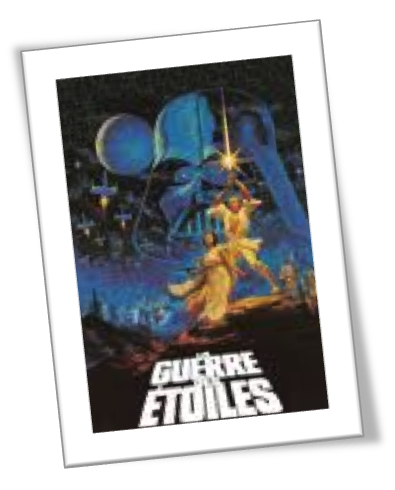
\includegraphics[width=0.95\textwidth]{images/starwars.png}\\
  
\includegraphics[width=0.9\textwidth]{images/apocalypsenow.png}
\end{minipage}
&
\begin{minipage}{0.7\textwidth}
\begin{exoblock}
\begin{enumerate}
\item Choisissez un film (f1), ainsi que deux de ses acteurs (a1 et a2).
\item Choisissez maintenant un autre film (f2) dans lequel joue a1.
\item Un film est composé d'un titre, d'une année, d'un réalisateur, et d'une liste d'acteurs. Un acteur est composé d'un nom, d'une date de naissance, et de la liste des films dans lesquels il joue. \\
\end{enumerate}

\medskip
 Proposez ensuite un fichier XML et sa DTD associée permettant de représenter ces informations avec le moins de redondance possible.
\end{exoblock}
\end{minipage}
\end{tabular}

\end{frame}

\begin{frame}[containsverbatim, fragile]{En manque d'inspiration ?}

Harrison Ford et Larry Fishburne ont tous les deux joué dans Apocalypse Now (1979, réalisation de Francis Ford Coppola).\\

Harrison Ford a également joué dans Star Wars (1977, réalisation de George Lucas).\\


\begin{tabular}{cc}
\begin{minipage}{0.45\textwidth}
 \begin{figure}
    
\includegraphics[width=0.5\textwidth]{images/fishburne.png}
    \caption{Larry Fishburne (n\'e le 30/07/1965)}
  \end{figure}
\end{minipage}
&
\begin{minipage}{0.45\textwidth}
 \begin{figure}
    
\includegraphics[width=0.5\textwidth]{images/ford.png}
    \caption{Harrison Ford (né le 13/07/1942)} \end{figure}
\end{minipage}
\end{tabular}



\prof{f1 : Apocalypse Now, 1979, réalisation de Francis Ford Coppola\\
a1 : Harrison Ford (colonel Lucas)\\
a2 : Larry Fishburne (Tyrone «Clean» Miller)\\
f2 : Star Wars, 1977, George Lucas}

\end{frame}



\begin{frame}[containsverbatim, fragile]{Remu-m\'eninges au cinéma...}

\begin{tabular}{cc}
\begin{minipage}{0.2\textwidth}
  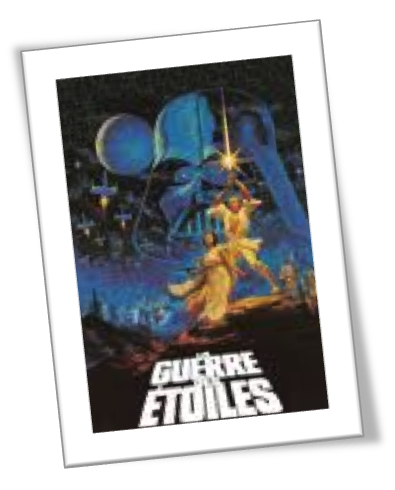
\includegraphics[width=0.95\textwidth]{images/starwars.png}\\
  
\includegraphics[width=0.9\textwidth]{images/apocalypsenow.png}
\end{minipage}
&
\begin{minipage}{0.7\textwidth}
Association plusieurs-à-plusieurs entre les entités film et acteur :
\begin{itemize}
\item à un acteur sont associés plusieurs films
\item à un film sont associés plusieurs acteurs
\end{itemize}
\end{minipage}
\end{tabular}


Le problème : \url{./codes/films_le_pb.xml}. \\

Une correction : \url{./codes/films_correction.xml}.\\

\end{frame}


\subsection{Quelques d\'etails}

\begin{frame}[containsverbatim]{Quelles valeurs peut prendre un attribut ?}

Un attribut peut contenir une liste de valeurs (NMTOKENS), les valeurs \'etant s\'epar\'ees par des espaces (pas d'autre s\'eparateur possible)

\begin{lstlisting}
<livre>
   <auteur>Carlo Batini</auteur>
   <auteur>Monica Scannapieco</auteur>
   <titre>Data quality: concepts, methodologies and techniques</titre>
   <annee>2010<annee>
</livre>
\end{lstlisting}

\begin{lstlisting}
<livre annee=2010 auteur="Batini Scannapieco">
   <titre>Data quality: concepts, methodologies and techniques</titre>
</livre>
\end{lstlisting}


\begin{lstlisting}
<livre annee=2010 autheur="Carlo Batini Monica Scannapieco">
   <titre>Data quality: concepts, methodologies and techniques</titre>
</livre>
\end{lstlisting}
\prof{4 tokens (4 valeurs)\\
Nous n'irons pas jusqu'aux MNTOKENS dans le cours (\`a n'utiliser que lorsque 
les valeurs sont s\'eparables par un s\'eparateur espace et qu'on veut mettre les infos dans un attribut). Contenu moins facile \`a r\'ecup\'erer par requ\^etage.
}
\end{frame}




\message{ !name(xml.tex) !offset(-1523) }
